\section{Implementation}
\label{sec:Implementation}

\subsection{Frontend}
There are many mature SPA frameworks today, such as Vue.js, ReactJS, Angular.js, Angular, and so on. Since the author is familiar with Angular, the frontend part of the project is implemented using Angular, which comes with almost everything we need, from powerful templates to fast rendering, data management, HTTP services, form handling, and so much more. Moreover, Angular provides a UI component library called Angular Material,
which is inspired by Google Material Design. Angular Material components help in constructing attractive, consistent, and functional web pages and web applications while adhering to modern web design principles like browser portability, device independence, and graceful degradation. It helps in creating faster, beautiful, and responsive websites.

In our design, the user must register to log in before he can use the application, so the home page is the login page. Luckily, Angular provides multiple routing guards, and the CanActivate interface is a good way for us to implement our own authentication routing. In addition, as we mentioned in Section \ref{sec:Requirements>Non-Functional Requirements} Non-Functional Requirements, every form must be validated by the client side before being submitted to the server side. The Implementation of GUI is listed below:

\begin{enumerate}
  \item The ``Sign Up'' form requires the user to enter a unique and valid email, first name, last name, password, and confirmed password. The user can click the icon on the right of the password input to make his password visible or invisible. Also, the ``clear'' button on the left bottom corner is used to clear all inputs of the Sign-Up form. The user can also click the ``Log in instead'' button to be redirected to the ``Log In'' page if he already has an account. Figure \ref{fig:GUI signup} is the interface of the ``Sign Up'' page.

  \begin{figure}[htbp]
  \centering
  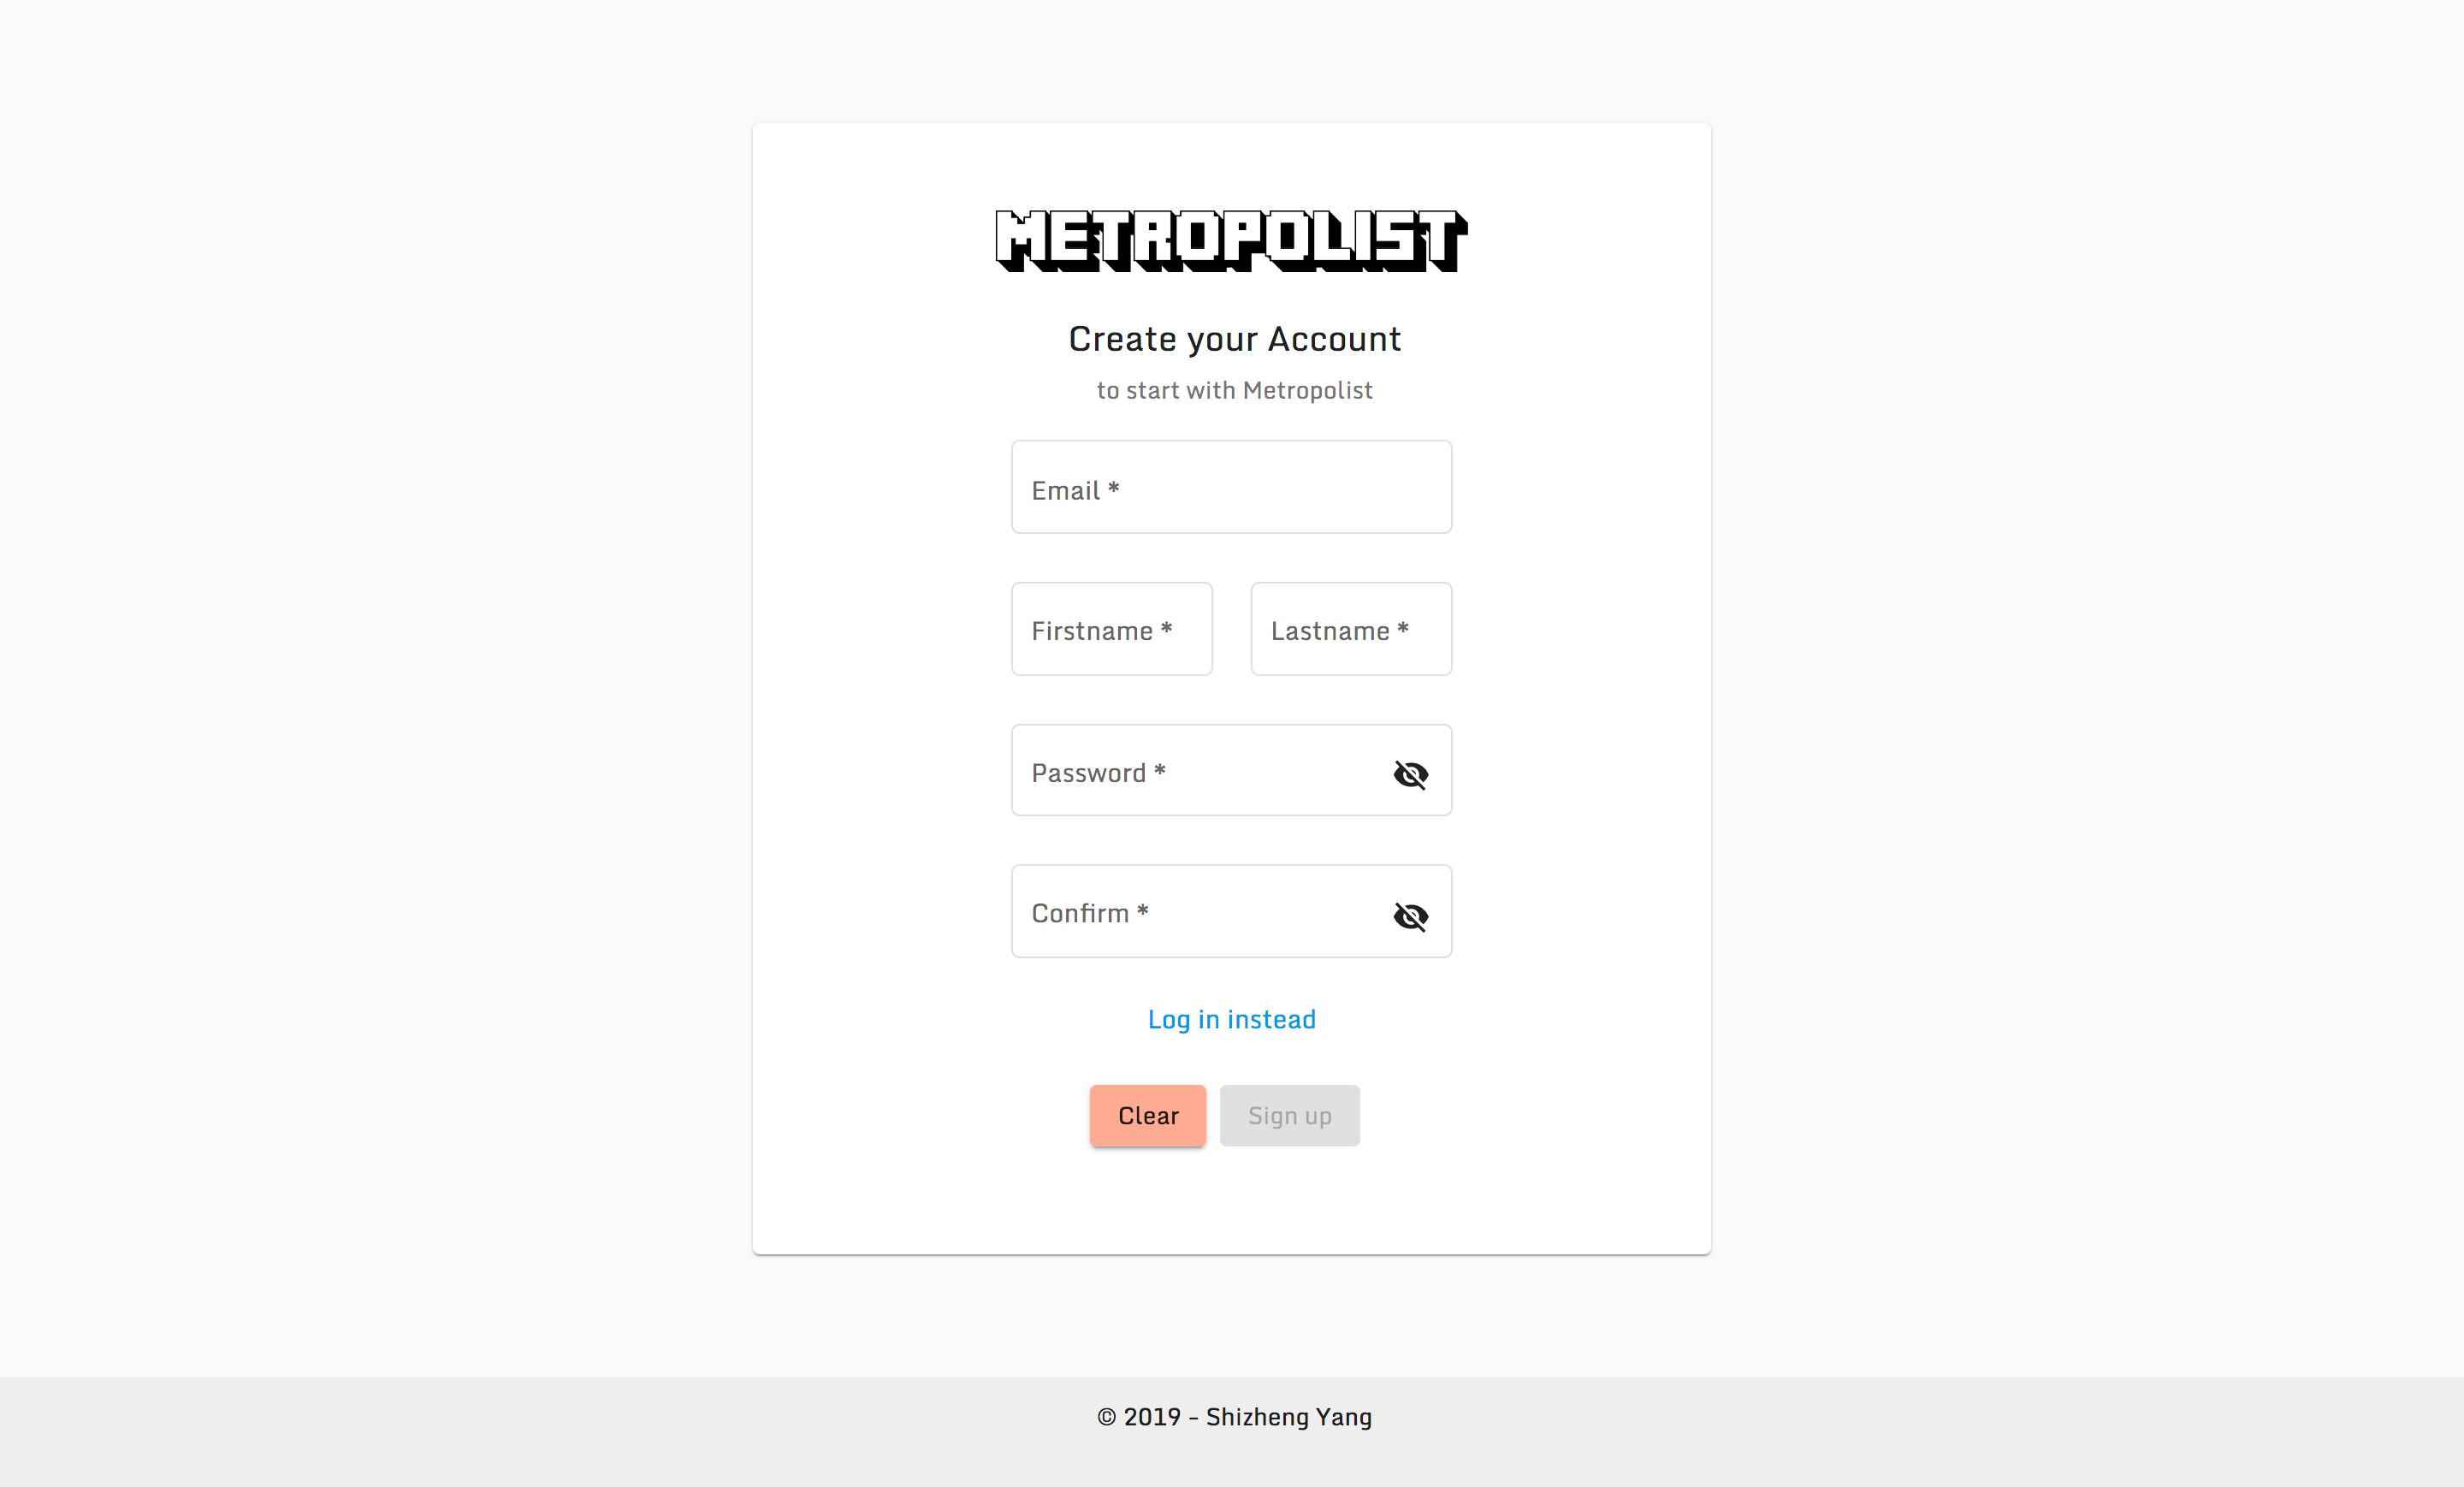
\includegraphics[width=\textwidth]{section04/assets/GUI-signup.png}
  \caption[GUI: Sign Up]{\label{fig:GUI signup}GUI: Sign Up}
  \end{figure}

  \item The ``Log In'' form requires the user to enter the email and the password. Also, the user can access to the Sign-Up page via the ``Create account'' button on the bottom. Figure \ref{fig:GUI login} is the interface of the ``Log In'' page.

  \begin{figure}[htbp]
  \centering
  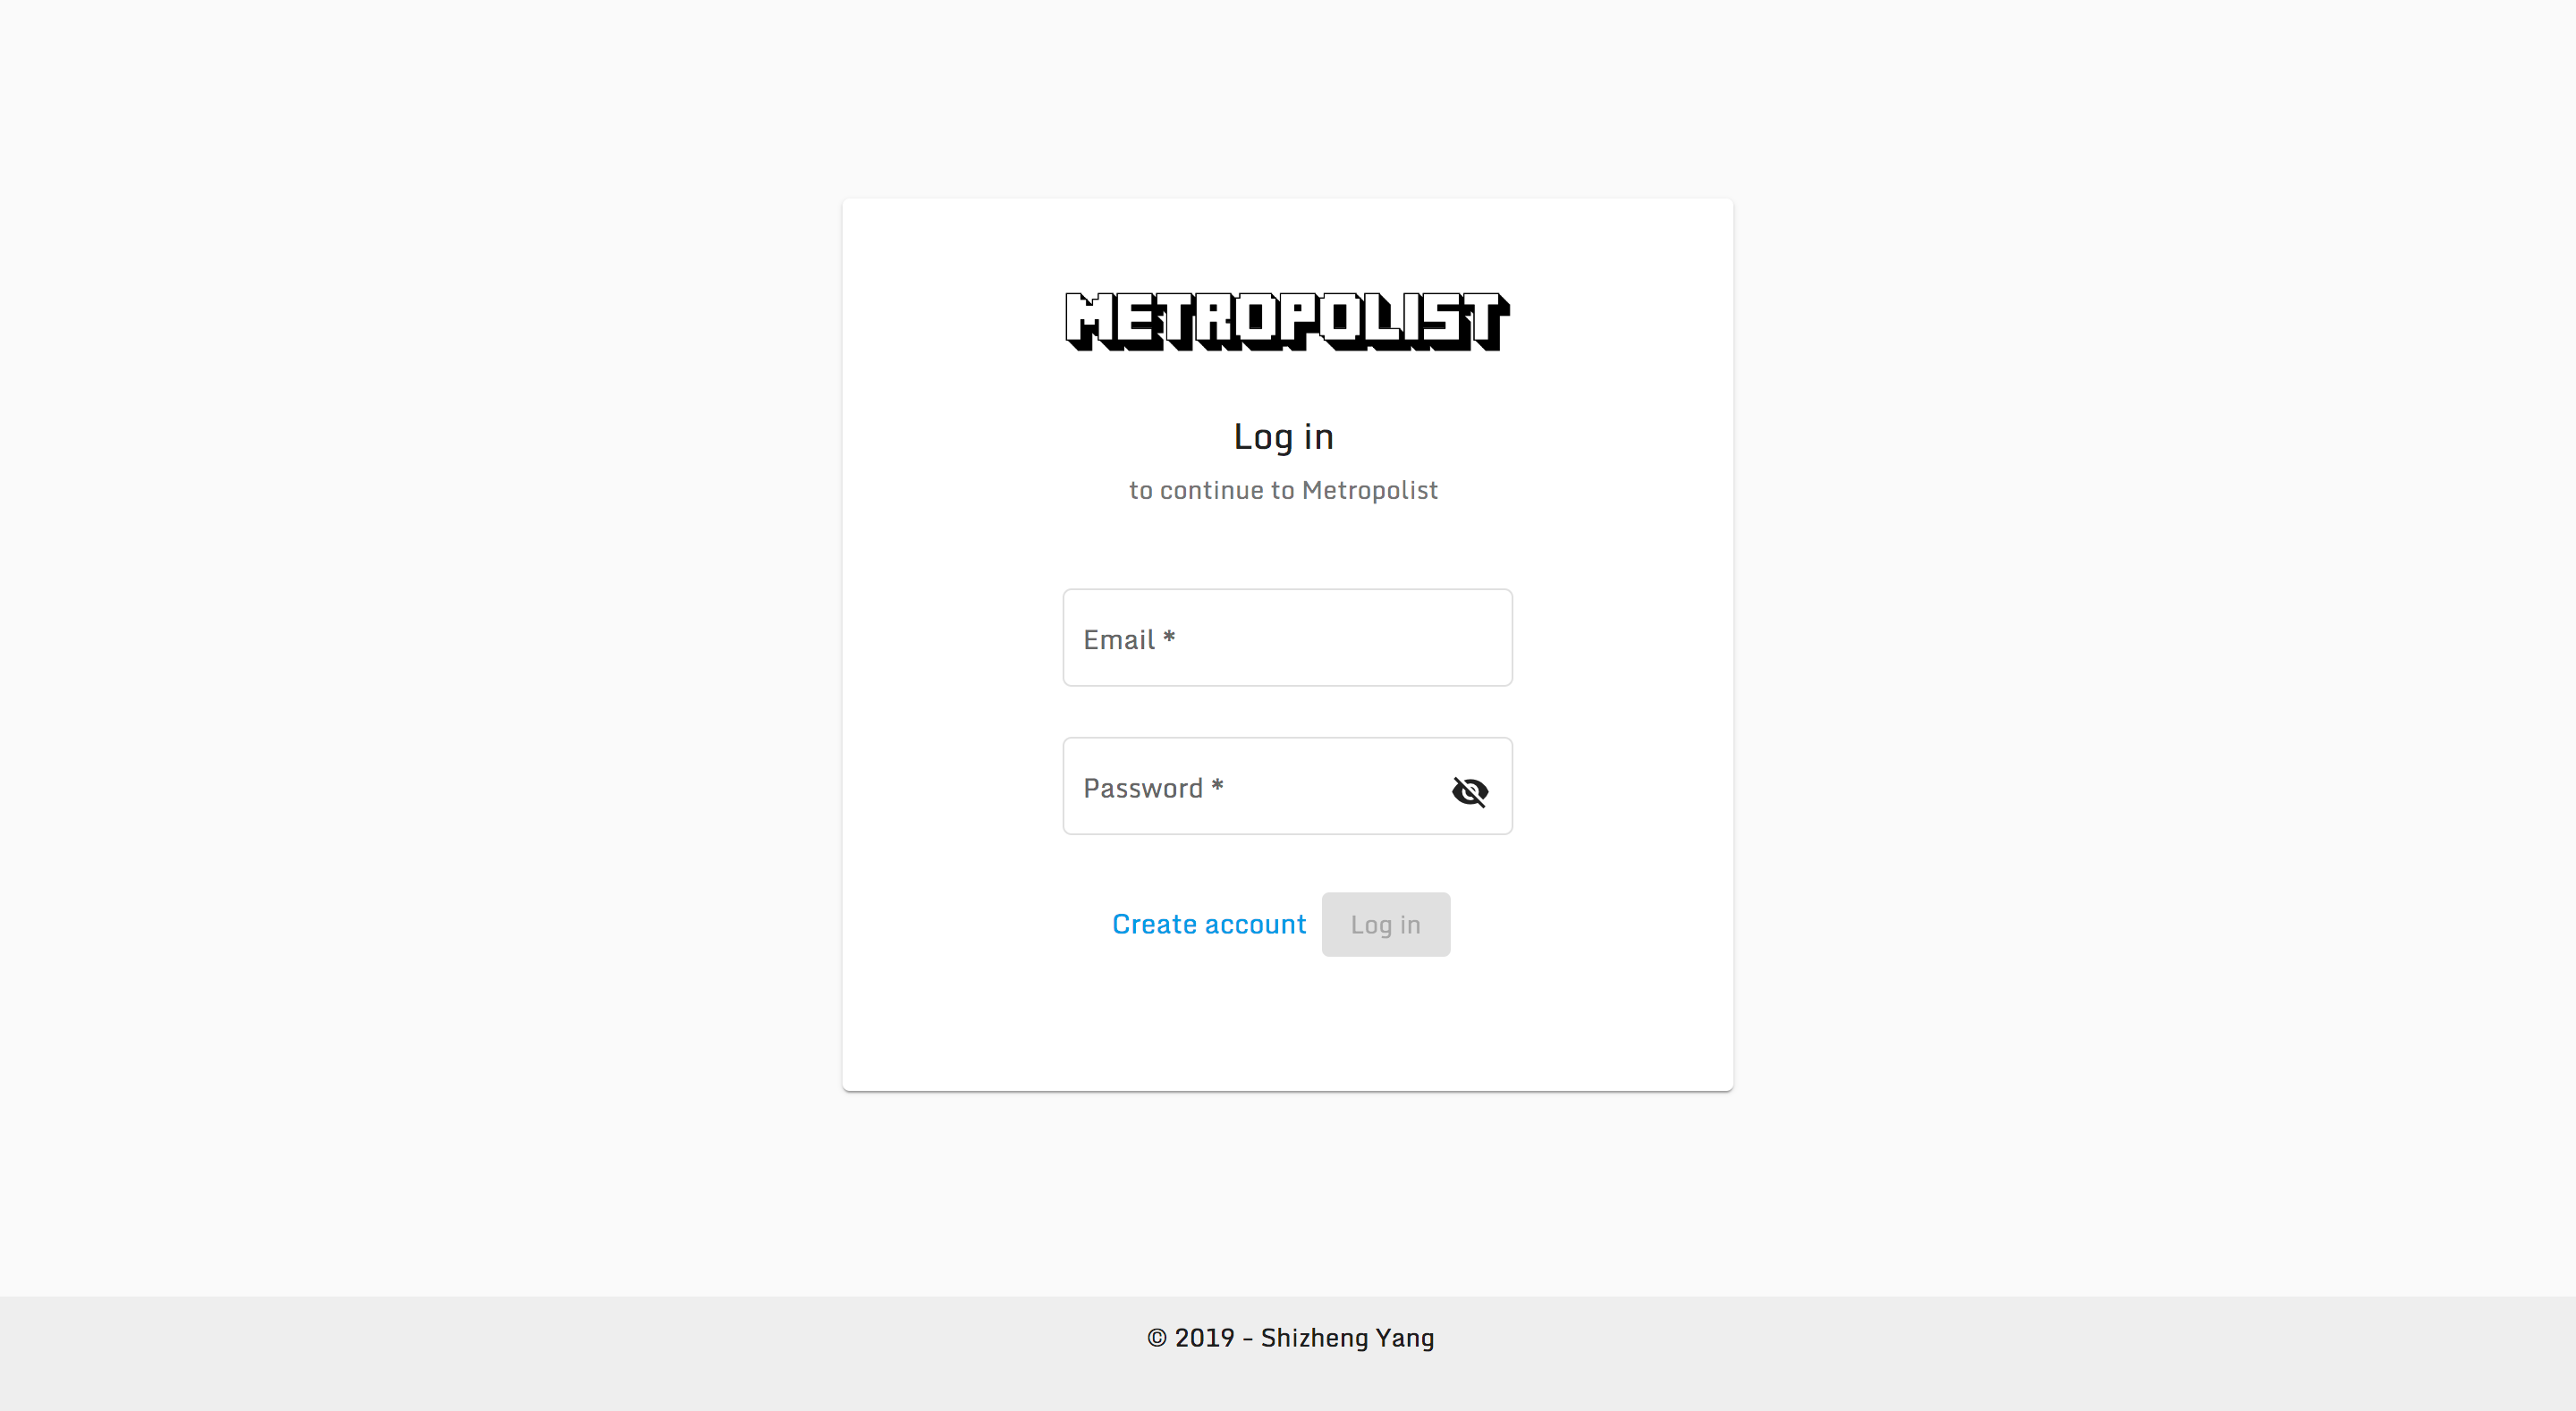
\includegraphics[width=\textwidth]{section04/assets/GUI-login.png}
  \caption[GUI: Log In]{\label{fig:GUI login}GUI: Log In}
  \end{figure}

  \item The ``Community'' page shows all the maps that can be viewed, which are marked by their own owners as ``isVisible.'' Besides, the user can filter maps using map name, owner's email, owner's first name, or owner's last name via the ``Filter'' on the left top corner. Figure \ref{fig:GUI community} is the interface of the ``Community'' page.

  \begin{figure}[htbp]
  \centering
  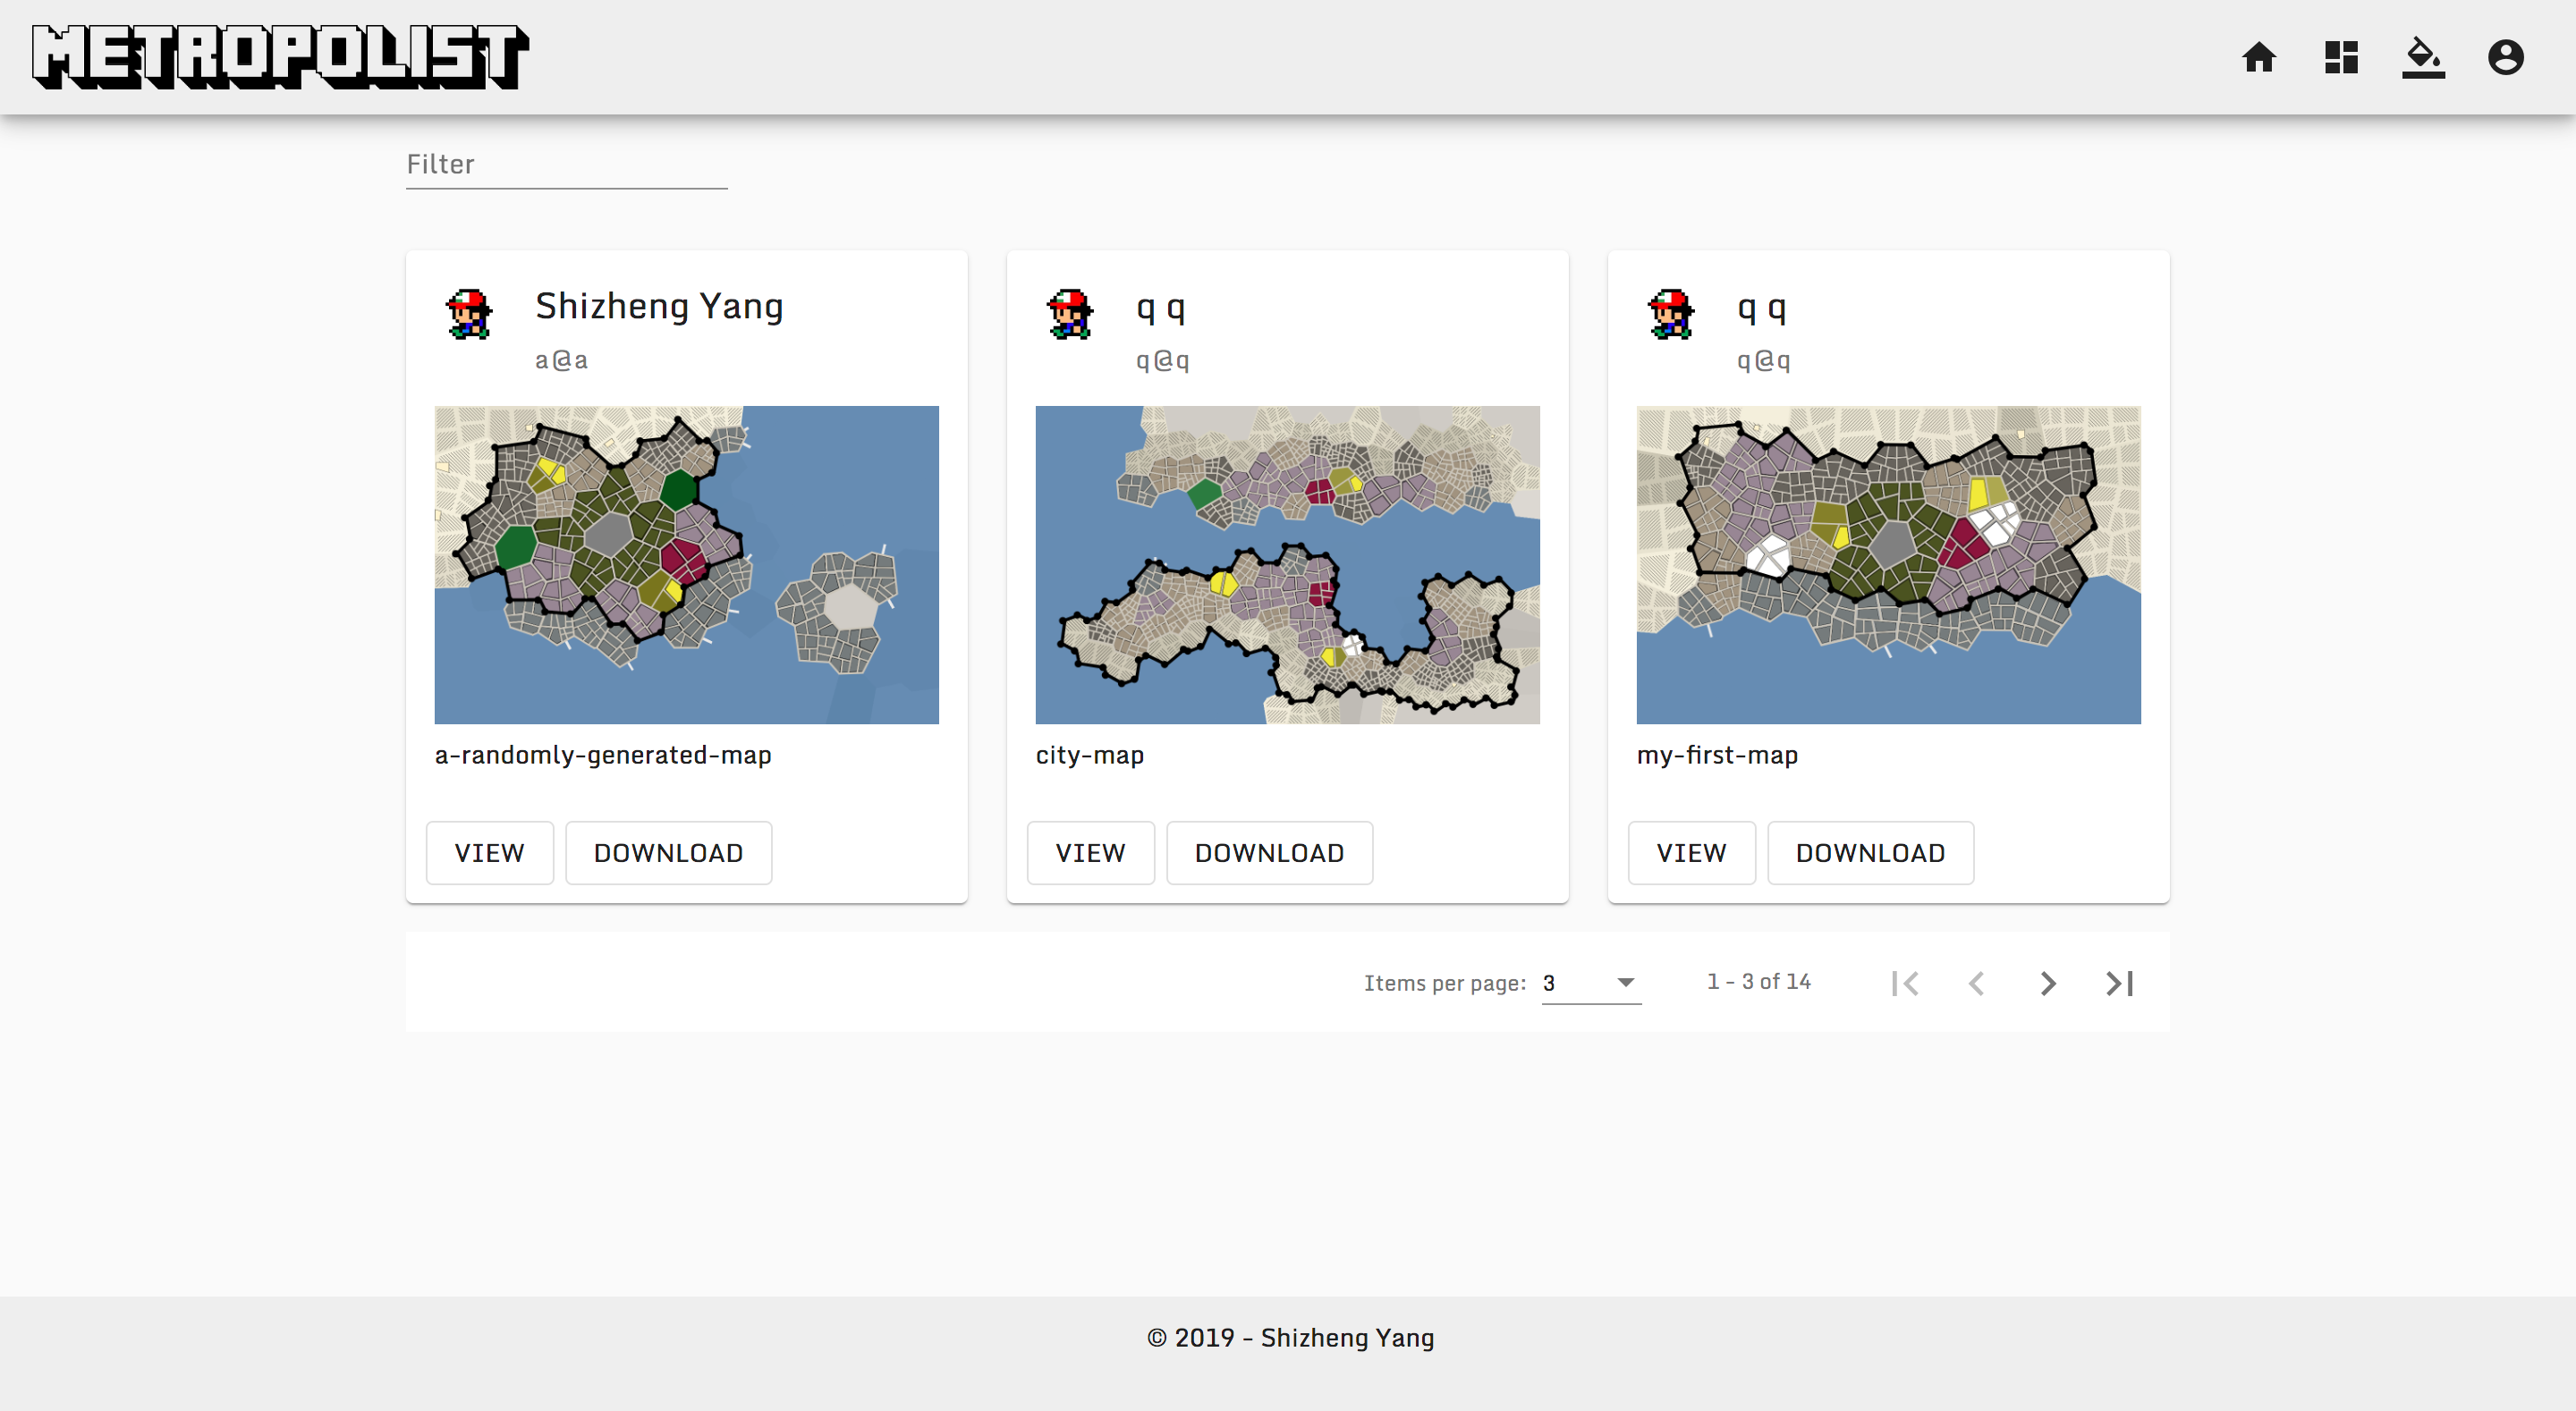
\includegraphics[width=\textwidth]{section04/assets/GUI-community.png}
  \caption[GUI: Community]{\label{fig:GUI community}GUI: Community}
  \end{figure}

  \item The ``User Dashboard'' page displays all the maps belong to the current user. The user can filter them using any information of maps via the ``Filter'' on the left top corner. The user can click on the header to perform the sorting of the corresponding map properties. Also, the user is allowed to make the map be visible or invisible by manipulating the slide of ``isVisible'', and edit, delete or download it via the three buttons in the ``Operation'' column. In addition, The button for creating a new map is in the lower right corner of the page. The user can enter a map name in the pop-up window after clicking it. Figure \ref{fig:GUI user dashboard} is the interface of the User dashboard page.

  \begin{figure}[htbp]
  \centering
  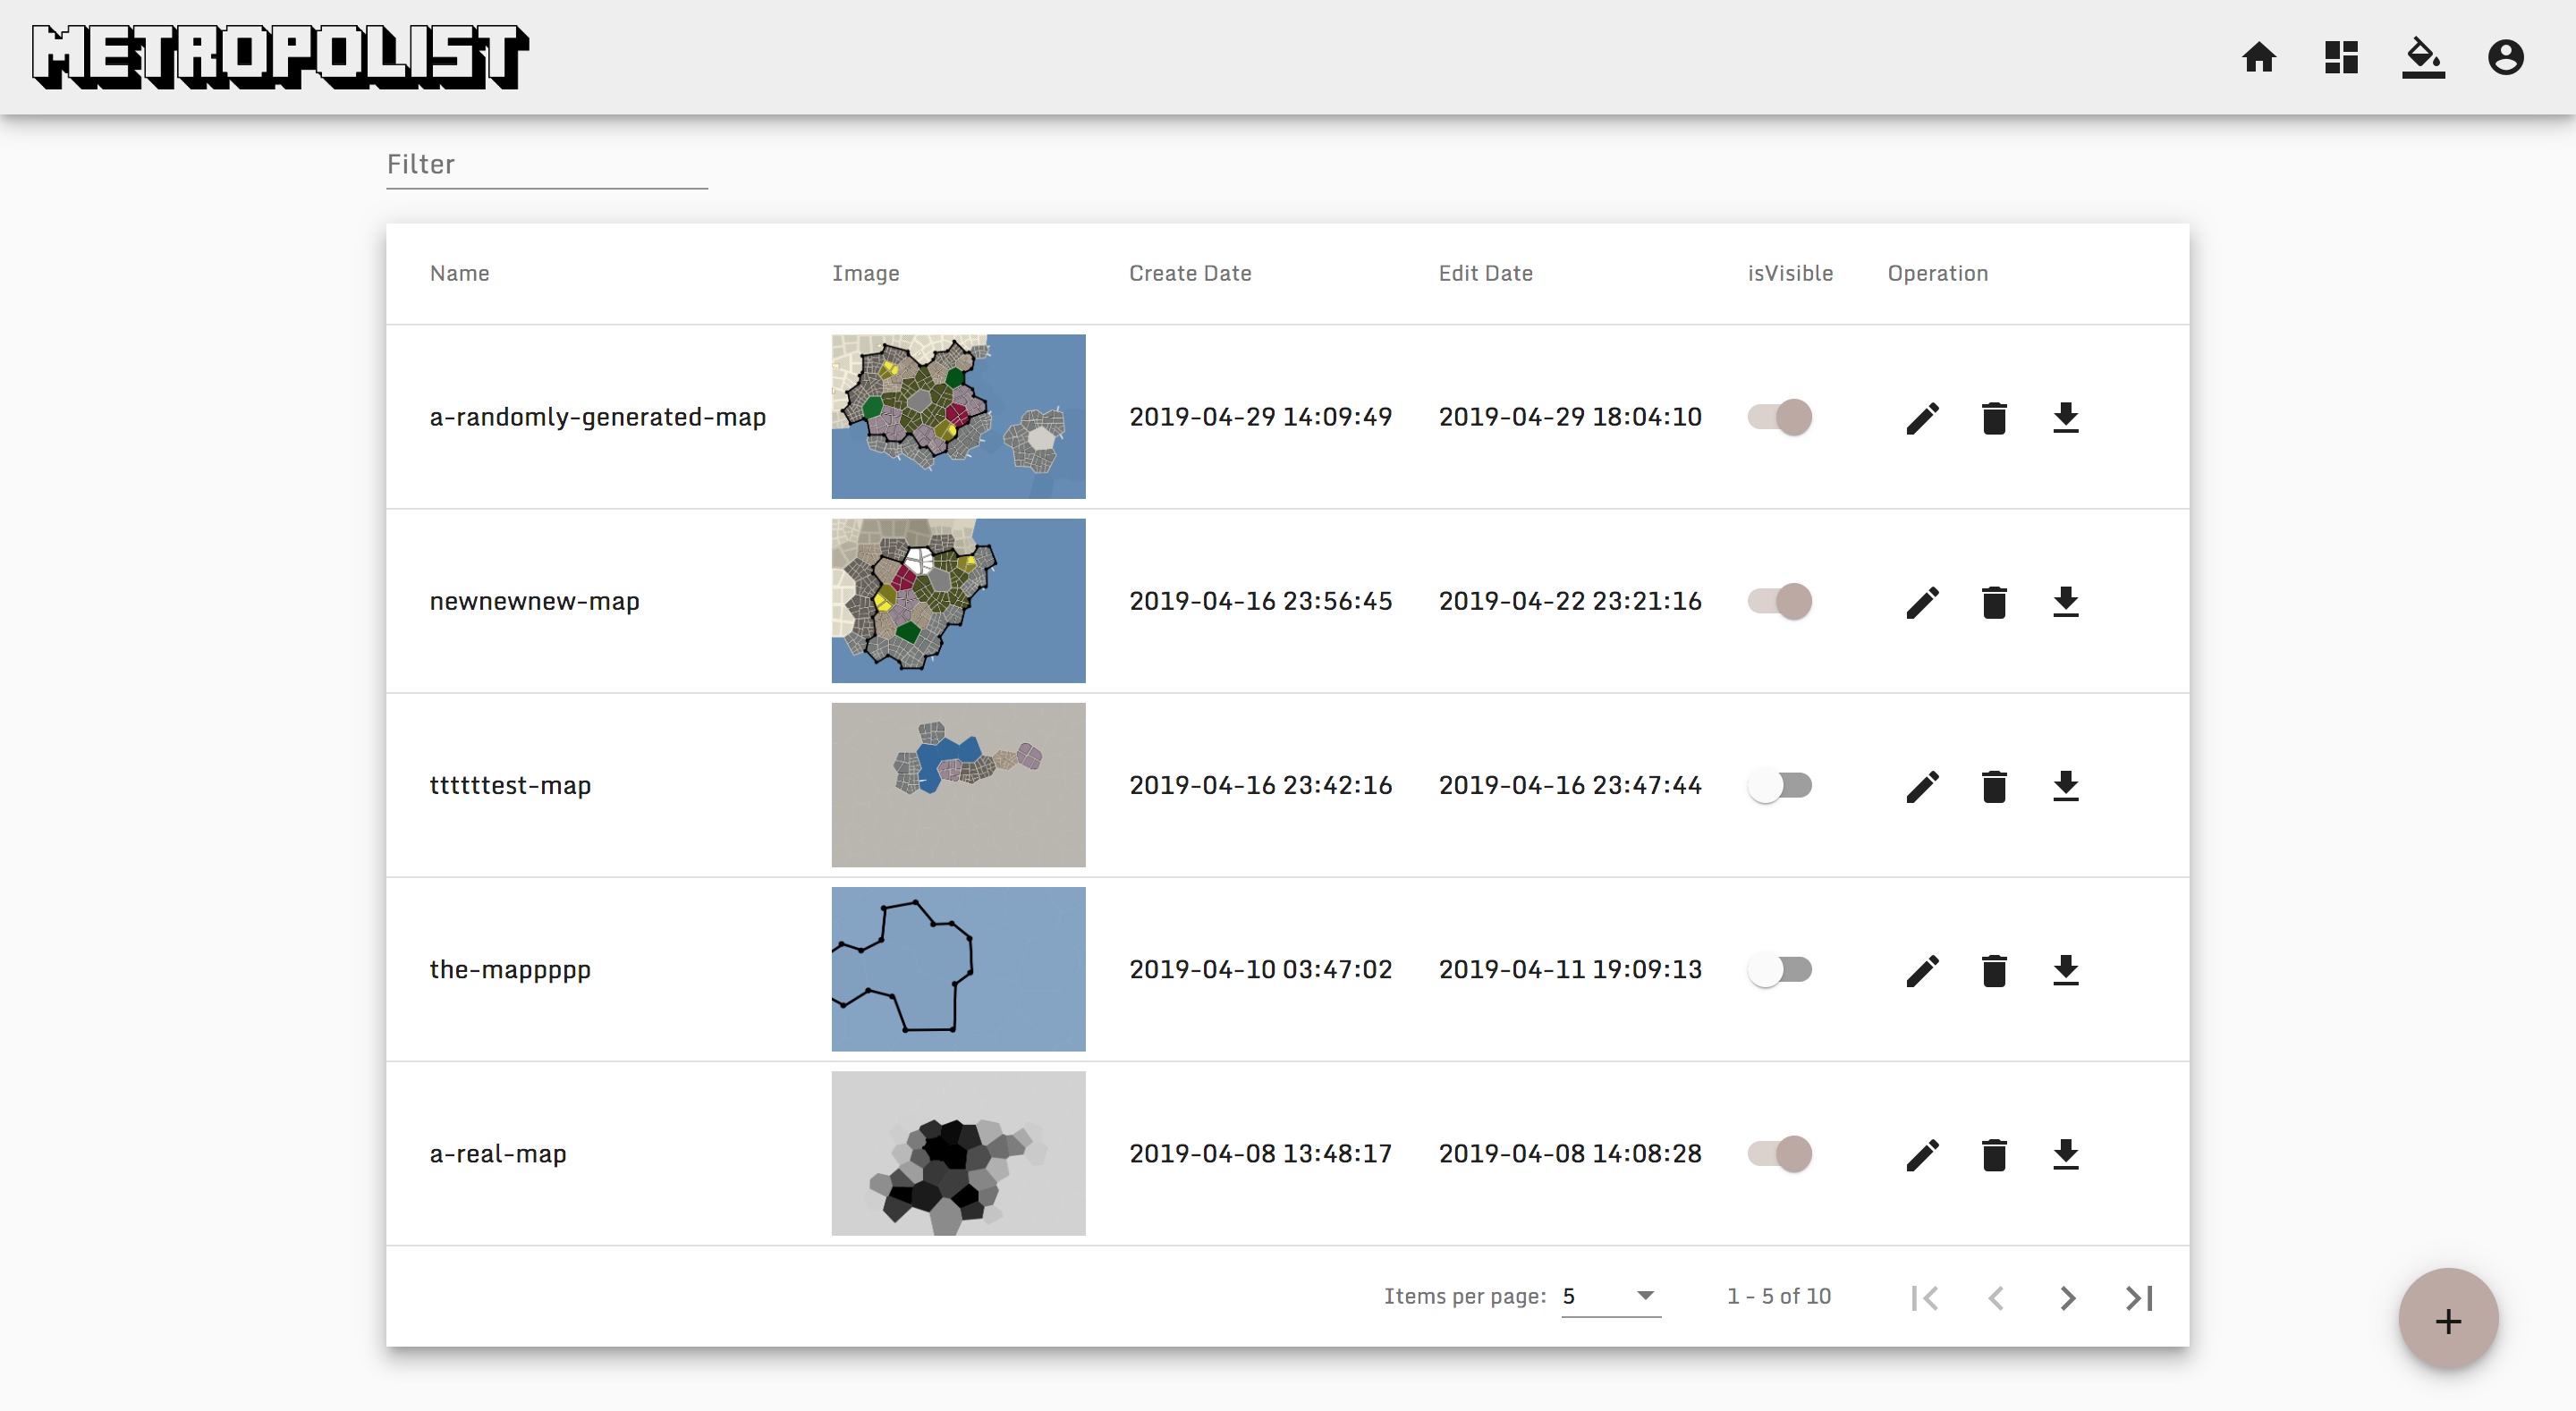
\includegraphics[width=\textwidth]{section04/assets/GUI-user.png}
  \caption[GUI: User Dashboard]{\label{fig:GUI user dashboard}GUI: User Dashboard}
  \end{figure}

  \item The ``Profile'' page allows the user to change his email, password, first name, or last name. By the way, before changing the password, the user must first enter the old password. After the verification is passed, the new password can be entered. Figure \ref{fig:GUI profile} is the interface of the Profile page.

  \begin{figure}[htbp]
  \centering
  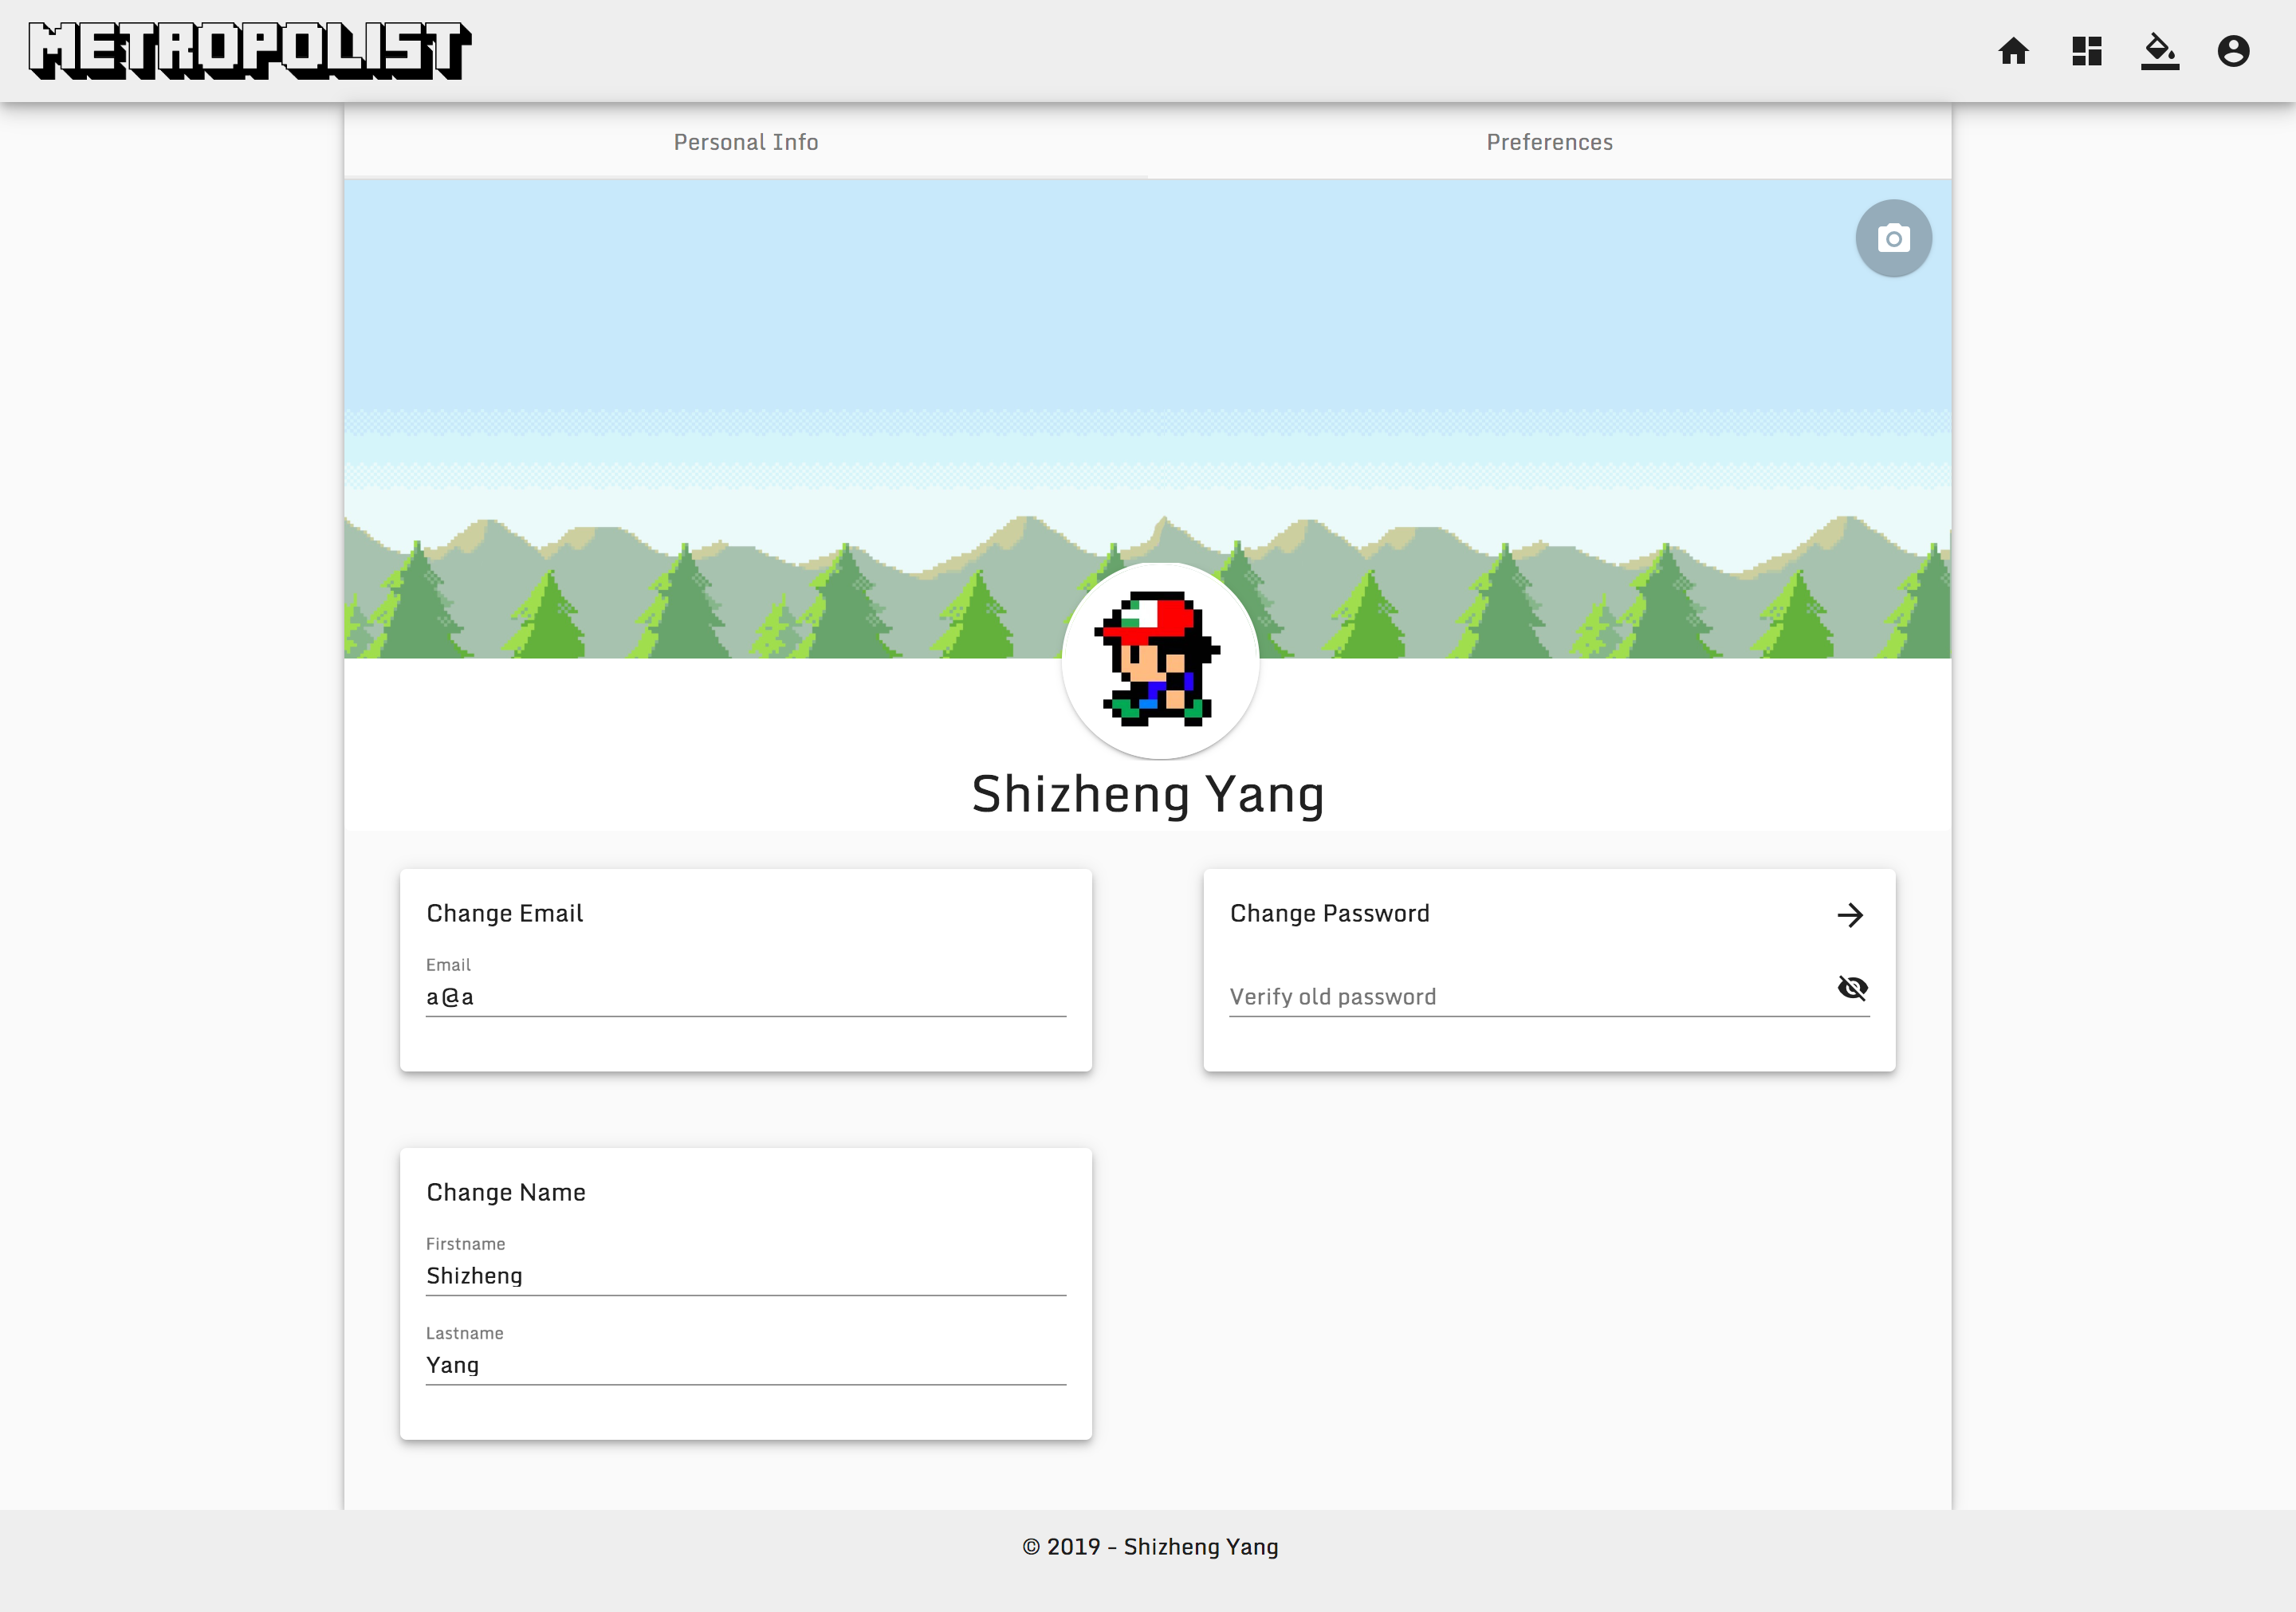
\includegraphics[width=\textwidth]{section04/assets/GUI-profile.png}
  \caption[GUI: Profile]{\label{fig:GUI profile}GUI: Profile}
  \end{figure}
\end{enumerate}

\subsection{Backend}
The backend comprises the server, database, and APIs. The server running on the author's computer, the database is powered by MongoDB, and the APIs are RESTful. And on this basis, we chose Express.js because it is a lightweight Node.js framework, which allows us to define routes of our application based on HTTP methods and URLs so that we can easily apply the REST API design to them very well. Also, it includes various middleware modules that we can use to perform additional tasks on the request and response.

To connect MongoDB to our Express application, we had to use an ORM to convert information from the database to a JavaScript application without SQL statements. ORM is short for Object Related Mapping, a technique that can be used to convert data among incompatible types. More specifically, ORMs mimic the actual database so we can operate within a programming language (e.g. JavaScript) without using a database query language (e.g. SQL) to interact with the database. For this application, we used Mongoose as the ORM, which is an object document modeling (ODM) layer that sits on top of the Node.js's MongoDB driver.

\subsection{Map Generator}
% Voronoi -> Lloyd's Relaxation -> D3 mouse events -> Layers: elevation, affluence,
\subsubsection{Polygons}
The first step is to render some polygons (cells). As we mentioned before in the design phase, we used the d3.voronoi library to implements Steven J. Fortune’s algorithm for computing the Voronoi diagram or Delaunay triangulation of a set of two-dimensional points. Figure \ref{fig:Voronoi polygons} is an example of random dots (red) and the polygons that result:

\begin{figure}[htbp]
\centering
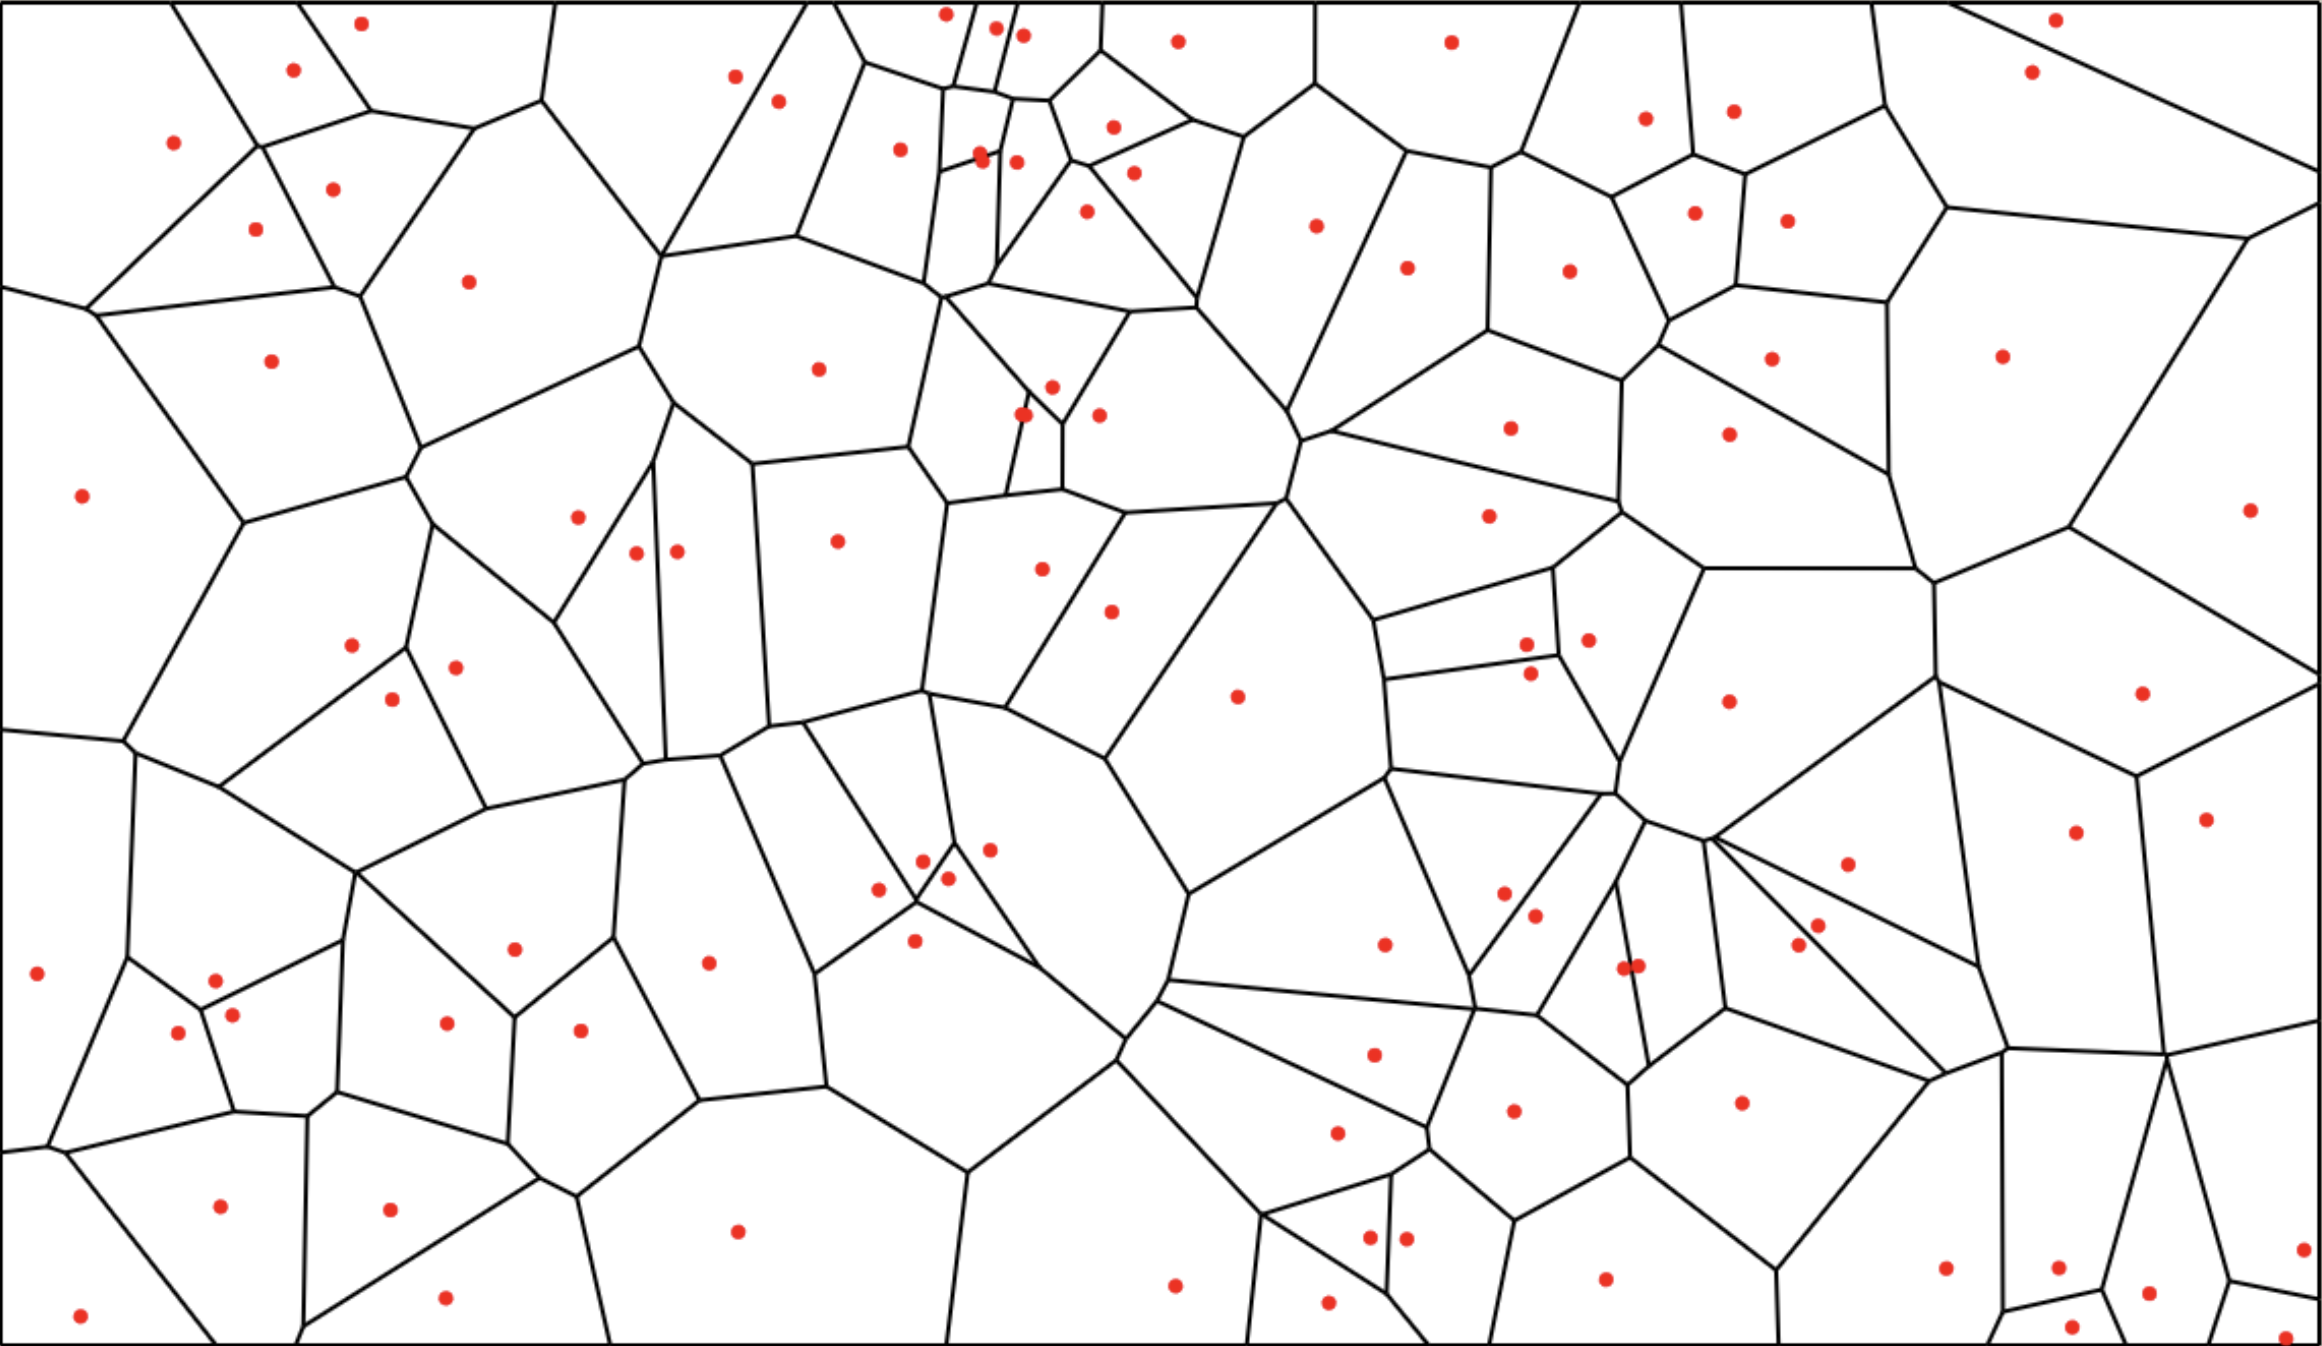
\includegraphics[width=\textwidth]{section04/assets/Map-voronoi.png}
\caption[Voronoi polygons]{\label{fig:Voronoi polygons}Voronoi polygons}
\end{figure}

As we can see these random points tessellation is a little bit irregular, we wanted something closer to semi-randomness or quasi-randomness, not completely random points. So we approximated that by using a variant of Lloyd relaxation, also known as Voronoi iteration or relaxation, which is a fairly simple tweak to the random point locations to make them more evenly distributed. Lloyd relaxation replaces each point by the centroid of the polygon. The more iterations, the more regular the polygons get. Figure \ref{fig:Voronoi relaxed polygons} is the result after running approximate Lloyd relaxation 5 times:

\begin{figure}[htbp]
\centering
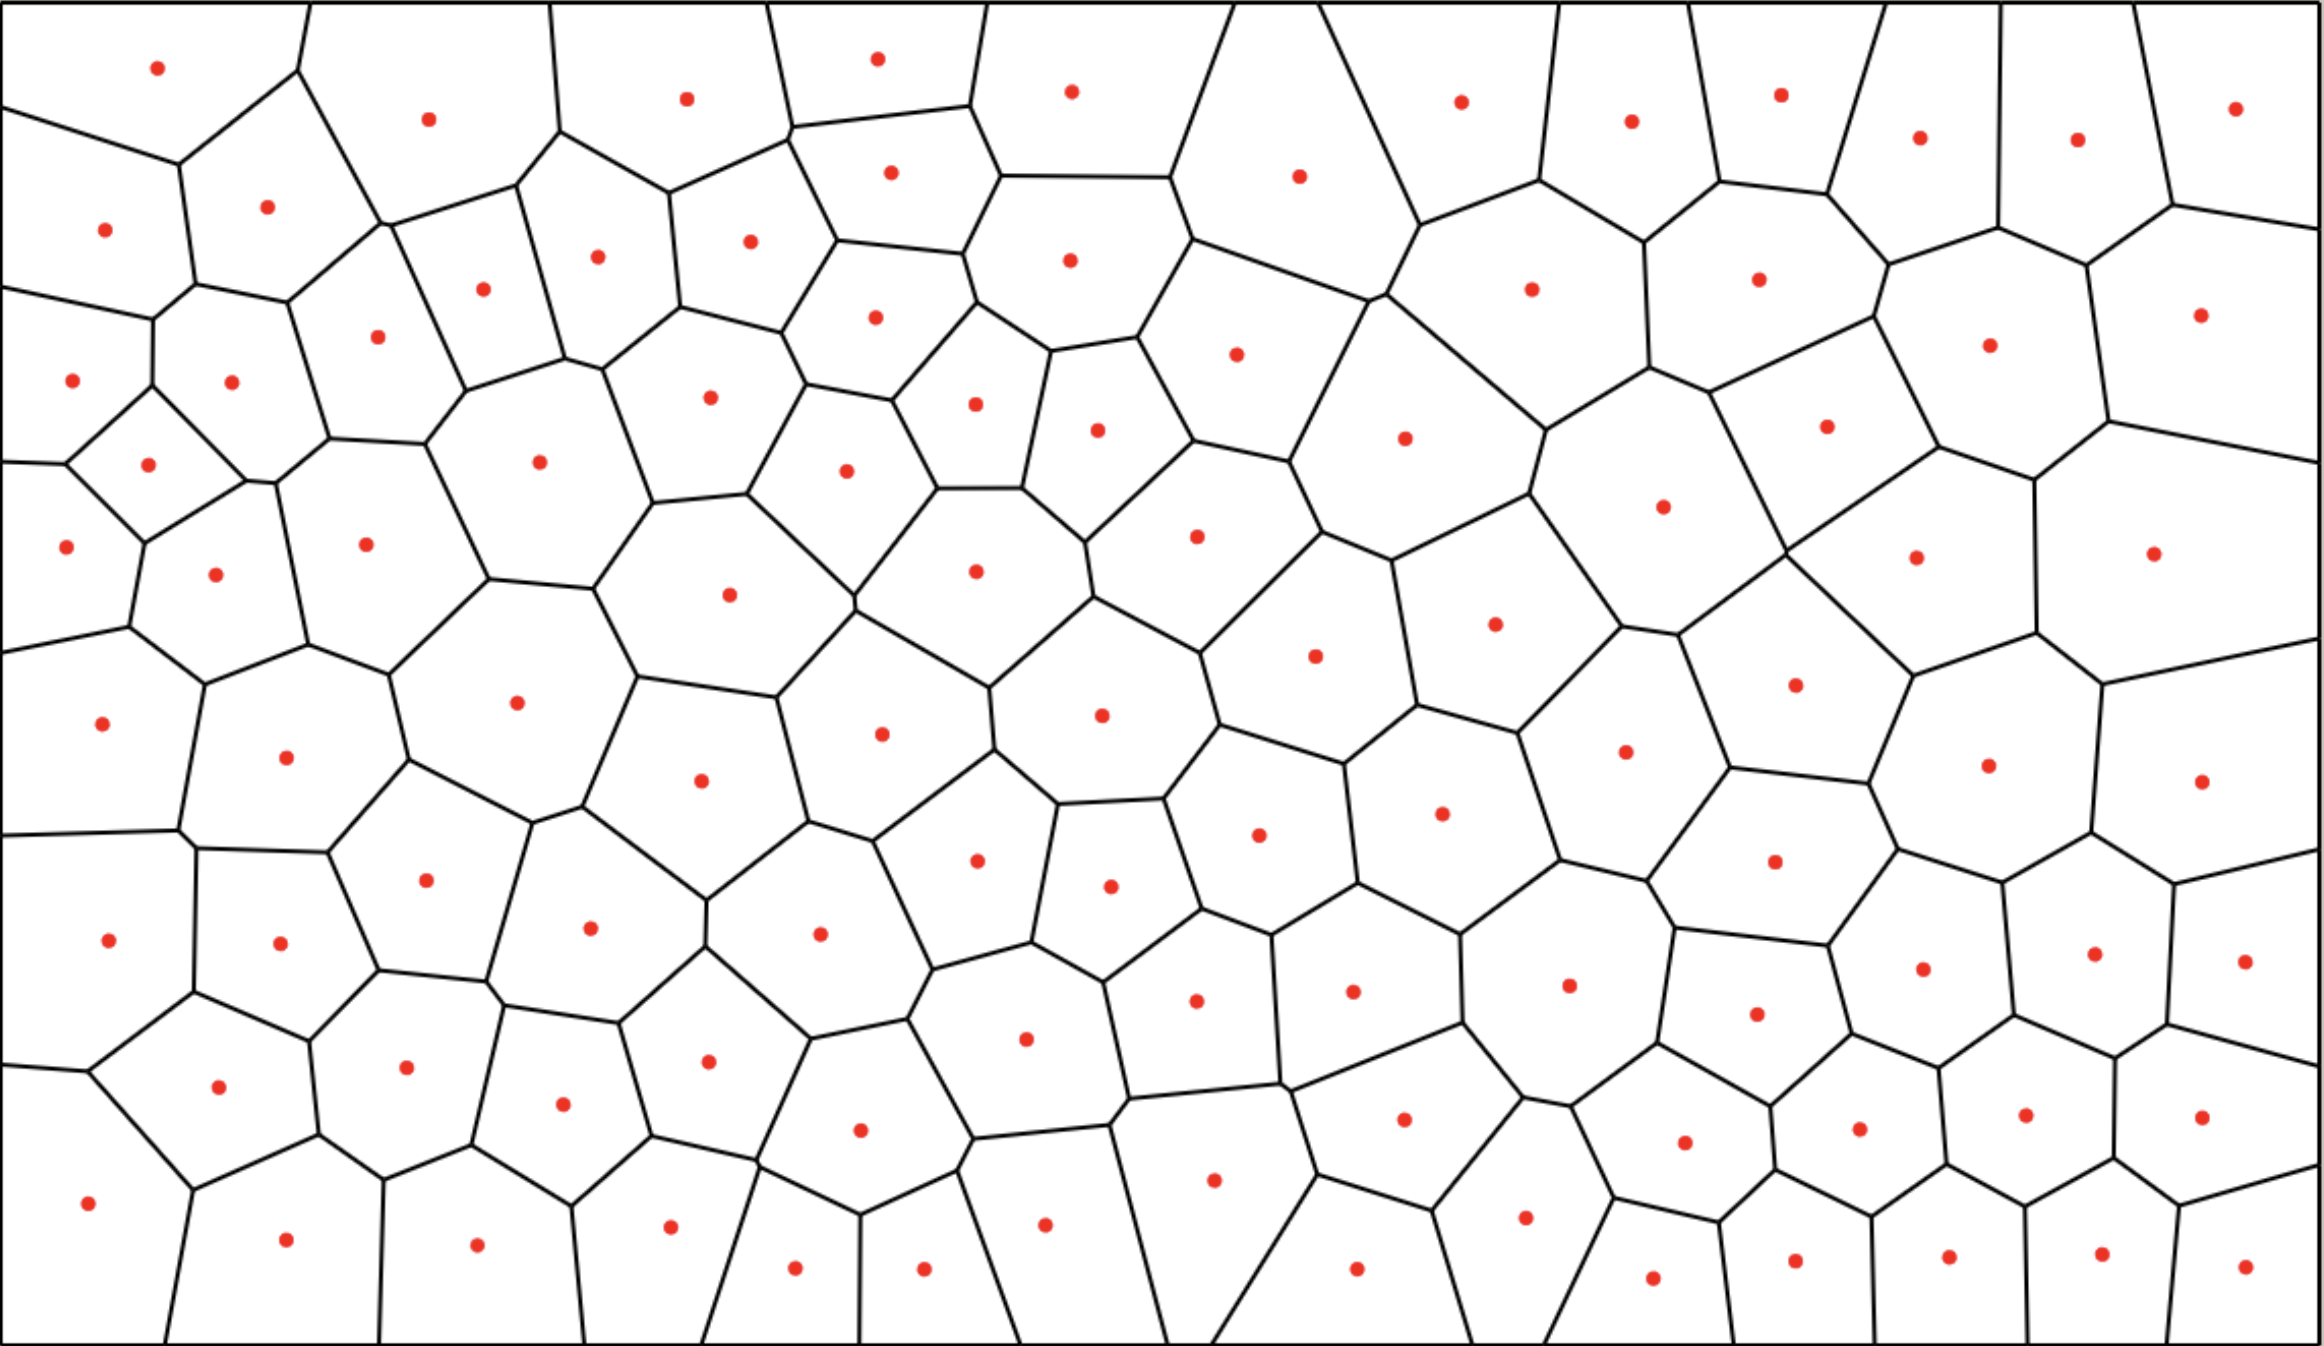
\includegraphics[width=\textwidth]{section04/assets/Map-voronoi-relaxation.png}
\caption[Voronoi polygons after 5 times of relaxation]{\label{fig:Voronoi relaxed polygons}Voronoi polygons after 5 times of relaxation}
\end{figure}

\subsubsection{Elevation}
As we mentioned in the map generator design phase, the map should be a height map, so we introduced the concept of ``elevation''. We called these dots that generate polygons as sites, and each site has a polygon corresponding to it. Then we derived the sites object from the d3.voronoi object, and assigned the ``elevation'' property to it, whose value from 0 to 1. Before making the height map, we defined the waterline, which is also from 0 to 1. If the value of elevation is greater than the waterline, the polygon represented by the site is the continent. Otherwise, it is water. Also, the darker the polygon is, the higher the elevation it represents. As the waterline rises, the continents with lower altitudes will be flooded and become water. So in the beginning, we set all the polygons to be continents and have an initial elevation that is 0.35. If the user wants to create water, then he should manually edit them. Figure \ref{fig:Height Map} is an example that divides the world into the continent and water:

\begin{figure}[htbp]
\centering
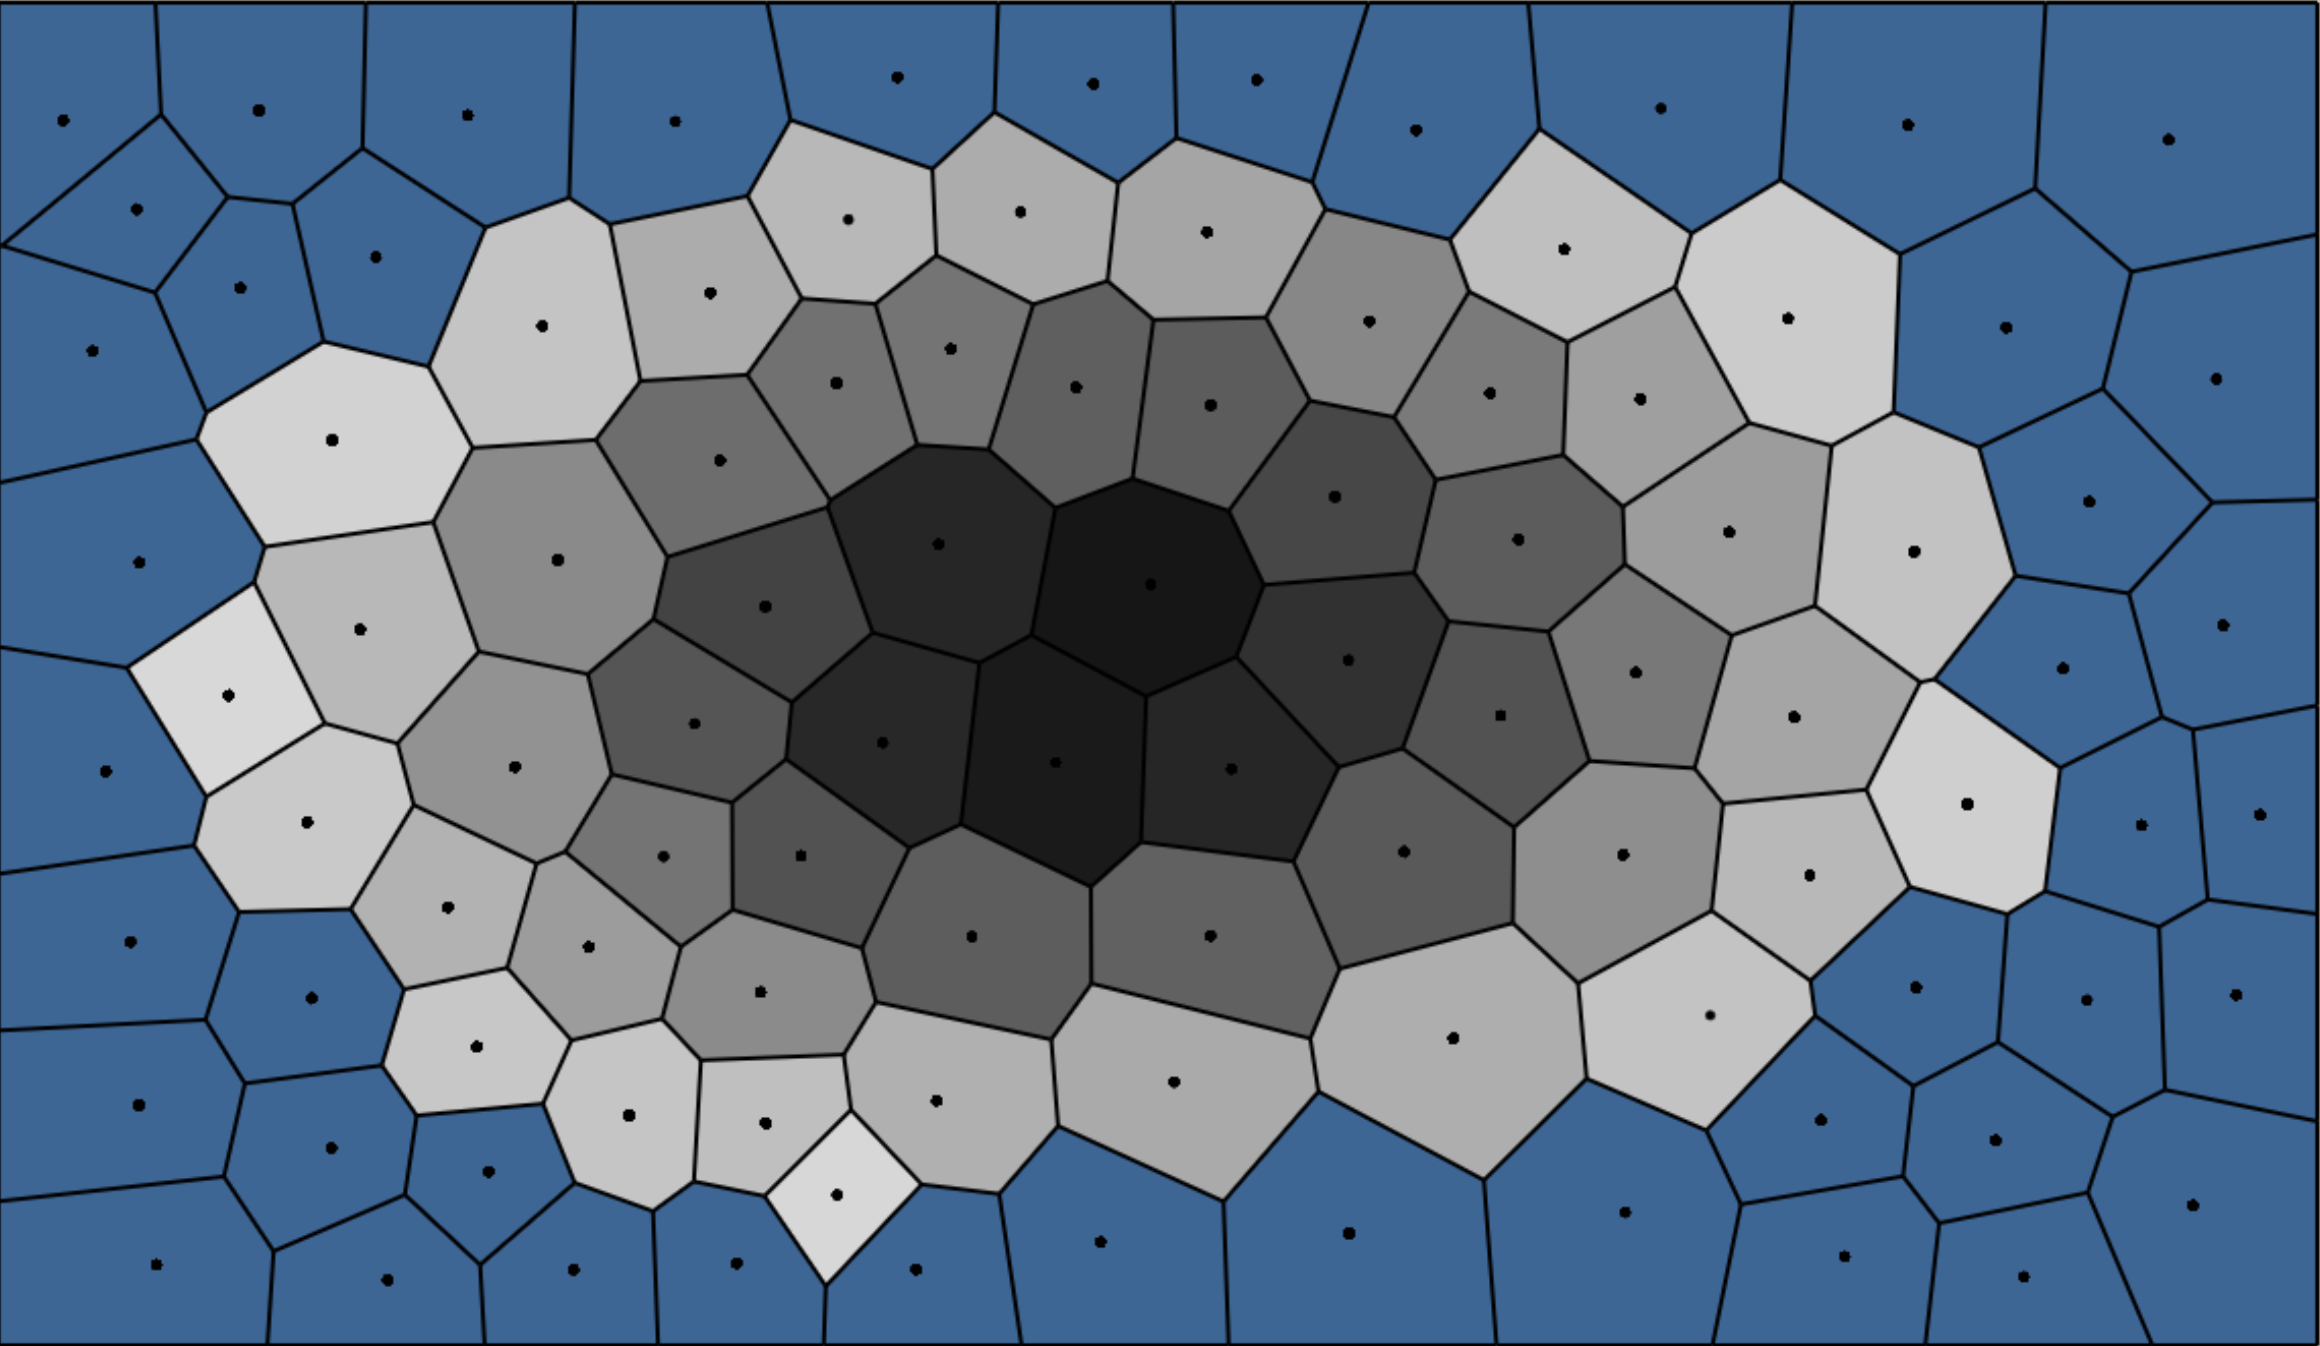
\includegraphics[width=\textwidth]{section04/assets/Map-heightmap.png}
\caption[Continent and Water]{\label{fig:Height Map}Continent and Water}
\end{figure}

\subsubsection{Contour Line}
We calculated the contour line of the map, which is determined by the elevation of each polygon, and is also based on the delaunay triangle, which comes from d3.voronoi.triangles.

These triangles link to each site, and each point has an elevation attribute. So when we set a value between 0 and 1, we loop every edge of every Delaunay triangle. If this value is between the elevation values of the two sites to which it is connected, we mark the point represented by this value and then connect all such points. Algorithm \ref{alg:draw contourline} describes the idea.

\begin{algorithm}
\caption{Draw contour lines for elevation X}
\label{alg:draw contourline}
\begin{algorithmic}
\REQUIRE $X \geq 0 \wedge X \leq 1$
\FOR{every triangle $T$}
\FOR{every edge $E1$, $E2$ in $T$}
\IF{$X \in E1 \& E2$}
\STATE Draw line from $E1$ to $E2$
\ENDIF
\ENDFOR
\ENDFOR
\end{algorithmic}
\end{algorithm}

We expect the user can determine the terrain by contour lines and use the tools we provided to edit the map. Figure \ref{fig:contour line} gives an example that draws four contour lines based on the value of waterline and couple elevation values: 0.25, 0.5, and 0.75.

\begin{figure}[htbp]
\centering
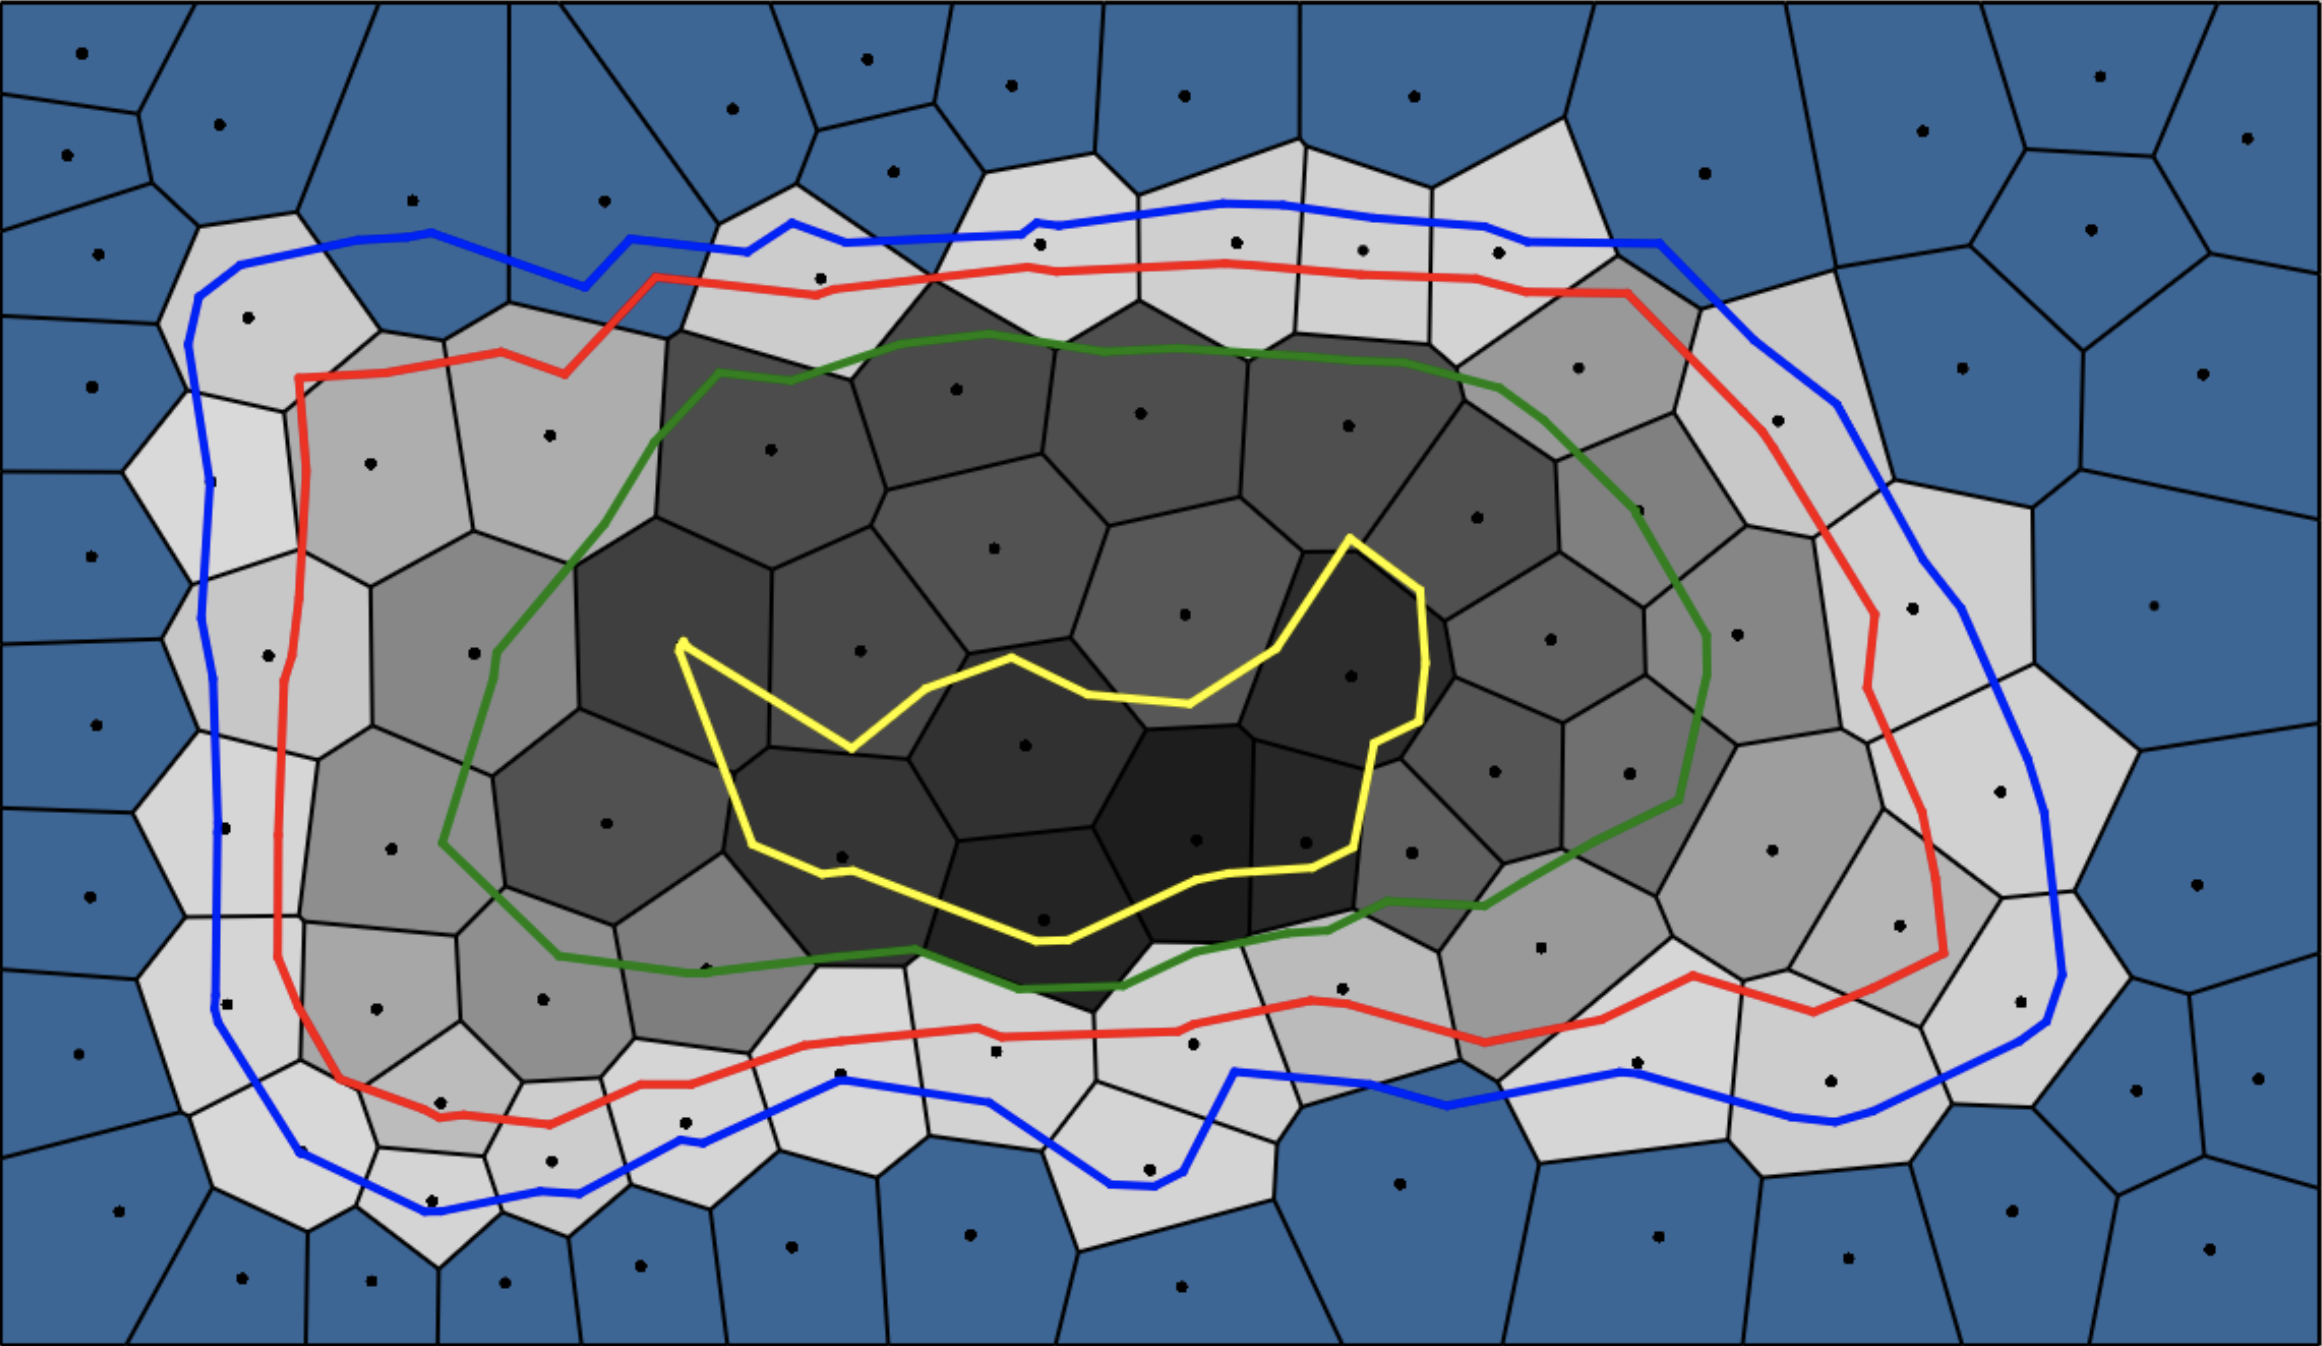
\includegraphics[width=\textwidth]{section04/assets/Map-contourline.png}
\caption[A map with contour lines]{\label{fig:contour line}A map with contour lines}
\end{figure}

\subsubsection{Soft Brush}
As mentioned in the previous section, the user needs to edit the map manually, so we provided some methods of operation, the most important of which is the soft brush. The soft brush is a circle that follows the mouse movement, and its role is to change the specific attribute values of all sites in the range.

In terms of elevation, the user can click and drag the soft brush to change the elevation of the selected sites accordingly. Generally speaking, the longer the distance is dragged, The more values are changed. The user first selects one of the two modes of ``increase'' or ``decrease''. Correspondingly, the attribute value of the site is increased or decreased under the operation of the soft brush. And the size of the soft brush can be enlarged or reduced by the mouse wheel.

\subsubsection{Layers}
Just like introducing the concept of elevation and assigning it to the sites, we then introduced the concepts listed below (including elevation):

\begin{enumerate}
  \item elevation: Represents the altitude of the area, from 0 to 1.
  \item affluence: Represents the wealth of the region (polygon), from 0 to 1.
  \item desirability: Represents the attraction of the region to people, from 0 to infinity.
  \item district: Displays different colors according to different regions; displays city walls.
  \item building: Displays buildings of specific districts.
\end{enumerate}

Each layer comes with two modes, ``view'' and ``edit''. Once the user has checked the edit option of a layer, its view option will also be checked; once the view option of a layer is unchecked, its edit option will also be unchecked.

The user can view them by checking different layers, and the layers can be superimposed on each other. For each polygon, we took the average of the sum of the currently selected layers color values as its background color.

\subsubsection{Types}
Based on the continent and water, we subdivided the regions on the continent into 13 types:

\subsubsection{Buildings}


\subsubsection{Streets}
